\documentclass{article}

\usepackage[spanish]{babel}
\usepackage[T1]{fontenc}
\usepackage[ansinew]{inputenc}
\usepackage[numbers,sort&compress]{natbib}
\usepackage{graphicx}
\usepackage{url}
\usepackage[numbers,sort&compress]{natbib}

\title {Movimiento Browniano}
\author{Anahi Llano}

\begin{document}

\maketitle

\section{objetivo}\label{obj}

\cite{baz} El objetivo de la practica fue: Examinar los efectos de la dimensi\'on con el tiempo de regreso al origen del movimiento browniano para dimensiones de 1 a 8 con incrementos lineales a uno, variando el n\'umero de pasos de la caminata con potencias de dos con exponente de 5 a 10 en incrementos lineales de uno, con 50 repeticiones del experimento para cada combinaci\'on.

\section{Metodolog\'ia}\label{met}

\cite{elis} A partir del c\'odigo en discord. Se realizaron modificaciones para llevar con \'exito la simulaci\'on, las cuales se observan en el c\'odigo ya cargado en github.
una vez realizada la simulaci\'on obtuve dos resultados:
723  (3)
1624 (2)
En los cuales se indica las veces que regreso y no regreso la part\'icula al origen, esto tomado en cuenta para calcular el tiempo de regreso.
En el archivo 'buenos', se encuentran los datos tomados en cuenta como son los pasos,la dimensi\'on y el tiempo de regreso de los 723 datos que son los relevantes, ya que no se contabilizan los escapes, para obtener este archivo se utiliz\'o un codigo similar a Clara. 
\cite{clara}

sink('buenos.txt')  
print(buenos).

Obteniendo as\'i el extracto de los datos. ya una vez teniendo los resultados se realiz\'o la gr\'afica correspondiente.
 
\section{Resultados}\label{res}

\cite{yo}
\centering
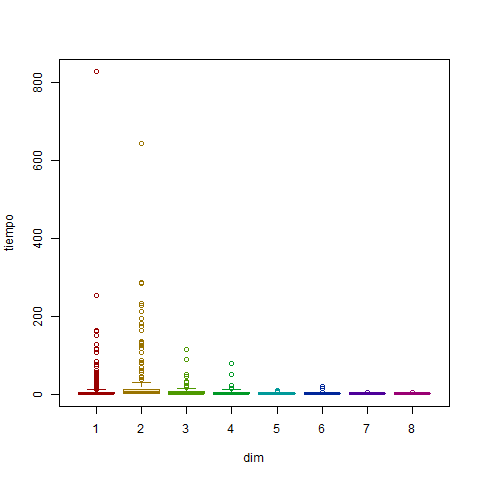
\includegraphics[scale=0.7]
{demo.png}
\begin{figure}\caption{Tiempo de regreso al origen.}
\end{figure}
\end{center}

\newpage

\section{Conclusion}\label{con}

Conforme se aumenta el largo en las 8 dimensiones sera m\'as dificil que una part\'icula regrese al punto de origen mientras mayor sea la dimensi\'on, de igual manera el tiempo que le tome en regresar sera mayor dependiendo de la dimensi\'on y el largo de esta.

\bibliographystyle{plainnat}
\bibliography{1}
\end{document}
 
